\begin{frame}{Warum Elektromobilität?}
	\pause
	\begin{itemize}[<+->]
        \item Umweltschutz gewinnt an Bedeutung
        \item 20\% aller \COO Emissionen aus Straßenverkehr, davon 60\% PKW
        \item Alternative: Elektrofahrzeuge
        \item Neue Art von Fahrzeug benötigt neue Informationssysteme
    \end{itemize}
\end{frame}

\begin{frame}{\COO Emissionen des Verkehrs in Deutschland \\1990 - 2004}
    \vspace*{\fill}
    \begin{figure}[h!]
       \centering
        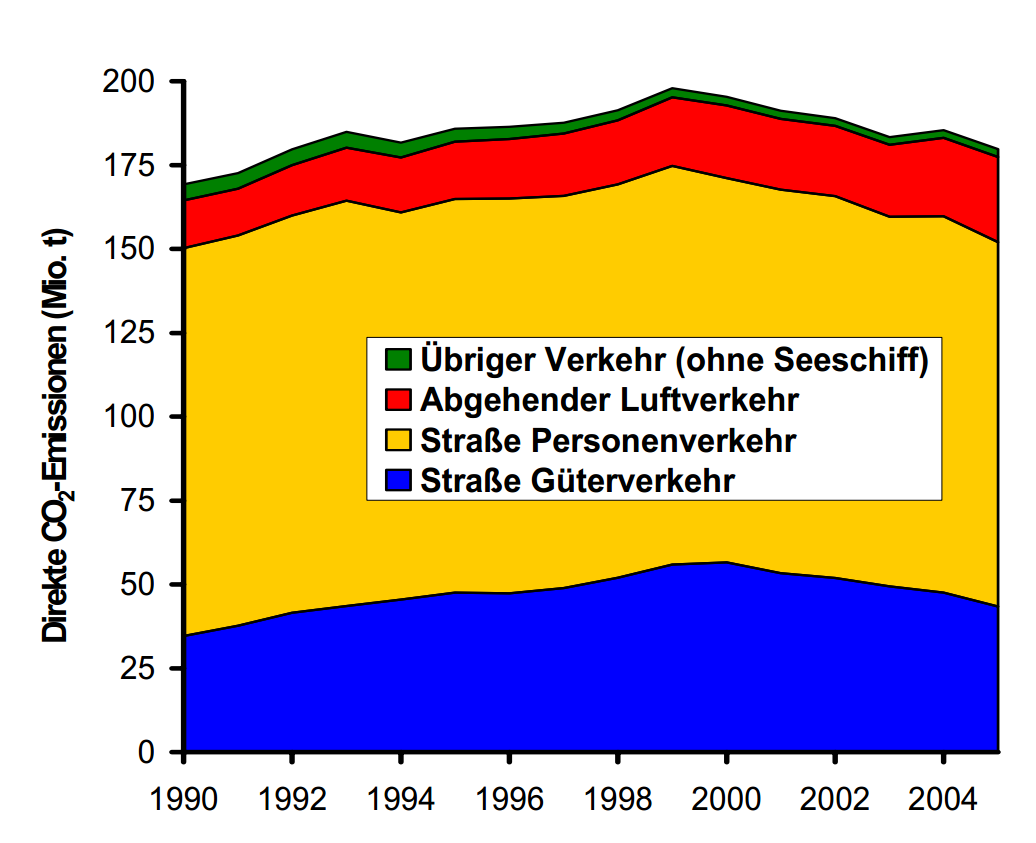
\includegraphics[width=0.66\textwidth,]{co2-emissionen.jpg}
    \end{figure}
    \vspace*{\fill}
\end{frame}



\begin{frame}{Warum neue Informationstechik?}
    \pause
    \begin{itemize}[<+->]
        \item Wachsende Komplexität der Informationstechnologie
        \item Zwischen 70 und 100 Steuergeräte in einem herlömmlichen Fahrzeug
        \item Zusätzliche Steuergeräte speziell für Elektrofahrzeuge
        \item Lösung: Neukonzipierung, Revolutionierung
    \end{itemize}
\end{frame}

\begin{frame}{Erwartete Entwicklung der Komplexität in Fahrzeugen 1955 - 2035}
    \vspace*{\fill}
    \begin{figure}[h!]
       \centering
       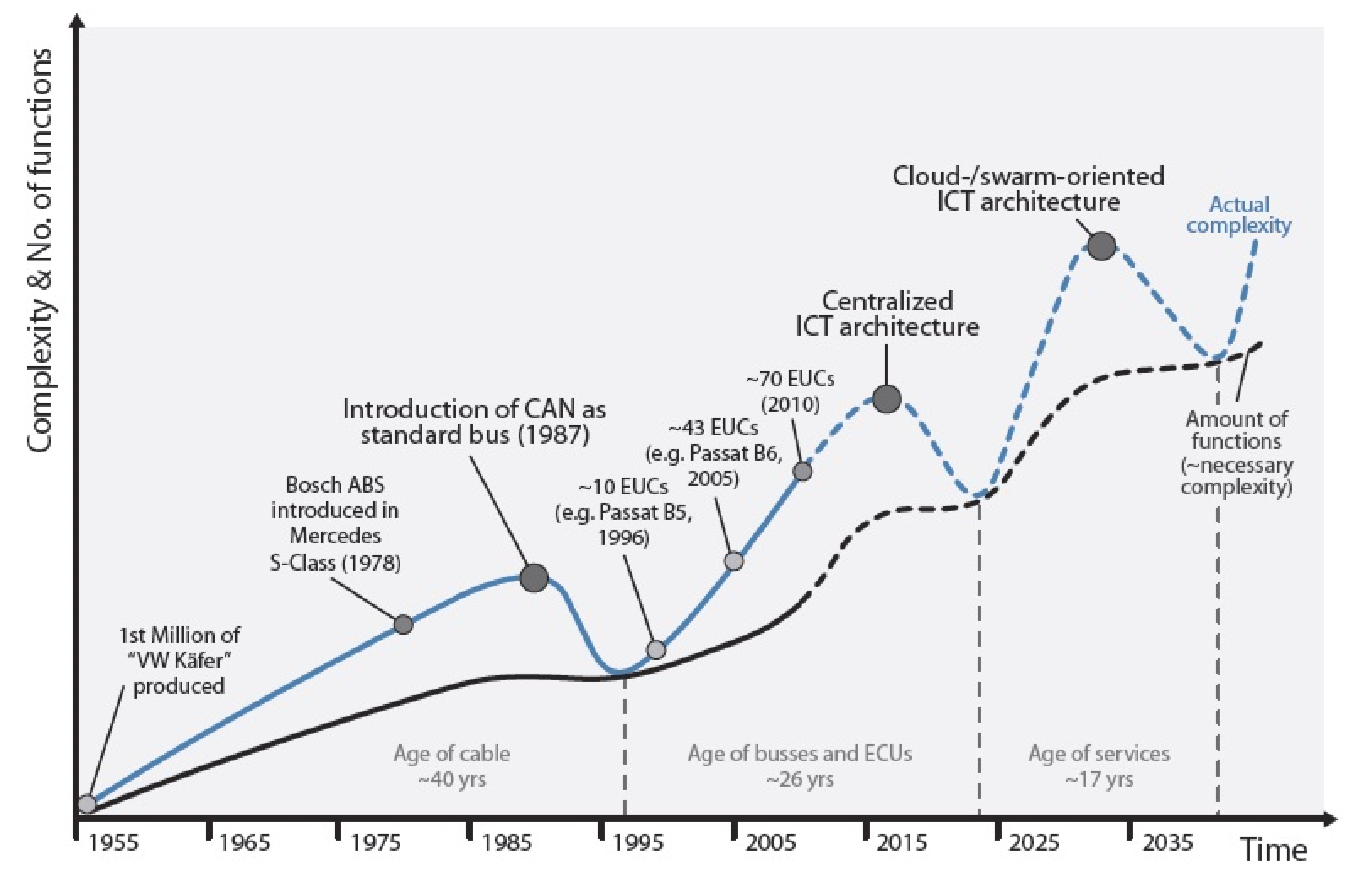
\includegraphics[width=0.66\textwidth,]{complexity.png}
    \end{figure}
    \vspace*{\fill}
\end{frame}